\[\sum_{l'}\Phi_{\alpha\beta}(l-l')=0\]
利用哈密顿正则方程,可以得到晶体震动位移满足的方程为
\[M\frac{d^2}{dt^2}u_l^\alpha=-\sum_{l',\beta}\Phi_{\alpha\beta}(l-l')u_{l'}^\beta\]
利用布洛赫定理,晶体的震动应有:
\[u_l^\alpha=e^{ik\cdot R_l}u_0^\alpha\]
由此可以得到退耦合的方程。\par
定义一个动力矩阵:
\[D_{\alpha\beta}(k)=\frac{1}{M}\sum_{l}\Phi_{\alpha\beta}(l)e^{-ik\cdot R_l}\]
由正格矢量与倒格矢量之间的关系可知:
\[D_{\alpha\beta}(k)=D_{\alpha\beta}(k+K_n)\]
最后求解得到特解(只有k标记的模式):
\[u_l^\alpha\sim\frac{1}{\sqrt{N}}e_k^\alpha e^{i(k\cdot R_l-\omega(k) t)}\]
其中
\[De_k=\omega(k)^2 e_k\]
不同的k得到不同的特解,可以用此特解作为基函数展开晶格振动的一般解:
\[u_l^\alpha=\frac{1}{\sqrt{NM}}\sum_{k,\sigma}e^{\alpha}_{k\sigma}Q_{k\sigma}e^{ik\cdot R_l}\]
对于复式晶格,假设每个晶胞内有r个原子,其动力学矩阵为:
\begin{equation}
D_{\alpha\beta}\left(\begin{array}{c}k\\s,s'\\\end{array}\right)=\frac{1}{\sqrt{M_sM_{s'}}}\sum_{l}\Phi_{\alpha\beta}\left(\begin{array}{c}l\\s,s'\\\end{array}\right)e^{-ik\cdot R_l}
\end{equation}
相应的动力学矩阵的本征方程为:
\begin{equation}
\sum_{\beta,s'}D_{\alpha\beta}\left(\begin{array}{c}k\\s,s'\\\end{array}\right)e^\beta_k(s')=w^2e^\alpha_k(s)
\end{equation}

\subsection{格波特性}
由于$\omega(k)$是动力矩阵的本征值,而动力矩阵具有周期性,因此$\omega(k)$也具有周期性:
\[\omega(k)=\omega(k+K_n)\]
由于做了一个点群操作之后,动力学矩阵之间相差一个相似变换,本征值不变,因此$\omega(k)$具有晶体所属点阵的点群的全部对称性:
\[\omega(k)=\omega(\beta k)\]
由于$\Phi(x)$是实函数,因此动力学矩阵满足:
\[D(k)=D(-k)^*\]
因此得到其本征值之间的关系:
\[\omega^2(k)=\omega^2(-k)\rightarrow \omega(k)=\omega(-k)\]
对于$w(0)=0$的格波称为声学模,对于$w(0)\ne0$的格波称为光学模。
简单晶格中,对于k=0,由于有:
\[D(0)=0\]
因此全部为声学模。对于确定的$w_\sigma(k)$本征值,声学模在长波限下满足条件:
\[\frac{e_{\Gamma\sigma}^\alpha(s)}{\sqrt{M_s}}=\frac{e_{\Gamma\sigma}^\alpha(s')}{\sqrt{M_s'}}\]
因此说明元胞内的原子之间是同向运动,对于每一个k,有三个独立的声学模。相应的光学模在长波极限下满足(2个原子的复式晶格):
\[\sqrt{M_1}e_{\Gamma\sigma}^\alpha(1)=-\sqrt{M_2}e_{\Gamma\sigma}^\alpha(2)\]
因此光学模代表晶胞内原子的质心不动,原子相对于质心的运动,对于每个k,有3r-3个光学模。
\subsection{简正坐标}
不同的k得到不同的特解,可以用此特解作为基函数展开晶格振动的一般解:
\[u_l^\alpha=\frac{1}{\sqrt{NM}}\sum_{k,\sigma}e^{\alpha}_{k\sigma}Q_{k\sigma}e^{ik\cdot R_l}\]
其中$Q_{k\sigma}$为简正坐标,引入正则动量
\[P_{k\sigma}=\frac{\partial L}{\partial \dot{Q_{k\sigma}}}=\dot{Q}_{k\sigma}^*\]
最后哈密顿量可以写为:
\[H=\frac{1}{2}\sum_{k\sigma}\{P_{k\sigma}^*P_{k\sigma}+Q_{k\sigma}^*Q_{k\sigma}\}\]
作傅立叶逆变换表明$Q_{k\sigma},P_{k\sigma}$是系统的集体坐标与动量。\par
对这个系统进行量子化,由对每个格点的正则量子化条件:
\[[p_l^\alpha,u_{l'}^\beta]=-i\hbar\delta_{l,l'}\delta_{\alpha,\beta}\]
\[[p_l^\alpha,p_{l'}^\beta]=0,[u_l^\alpha,u_{l'}^\beta]=0\]
可以推导得出对于集体坐标的正则量子化条件:
\[[P_{k,\sigma},Q_{k',\sigma'}]=-i\hbar\delta_{k,k'}\delta_{\sigma,\sigma'}\]
\[[P_{k,\sigma},P_{k',\sigma'}]=0,[Q_{k,\sigma},Q_{k',\sigma'}]=0\]
由于之前的哈密顿量不是谐振子系统的形式,做正则变换:
\[a_{k\sigma}=\sqrt{\frac{\omega_\sigma(k)}{2\hbar}}(Q_{k\sigma}-\frac{P_{-k\sigma}}{i\omega_\sigma(k)})\]
\[a_{k\sigma}^\dagger=\sqrt{\frac{\omega_\sigma(k)}{2\hbar}}(Q_{-k\sigma}+\frac{P_{k\sigma}}{i\omega_\sigma(k)})\]
那么系统的哈密顿量为:
\[H=\sum_{k,\sigma}\hbar\omega_\sigma(k)(a_{k\sigma}^\dagger a_{k\sigma}+\frac{1}{2})=\sum_{k,\sigma}H_{k,\sigma}\]
代表3N种不同$(k,\sigma)$的无相互作用的声子系统,总能量:
\[E=\sum_{k,\sigma}(n_{k,\sigma}+\frac{1}{2})\hbar\omega_\sigma(k)\]
说明晶格振动的激发状态。可以用3N个数$\{n_{k,\sigma}\}$来描述\par
声子是格波激发的量子,称为集体震荡的元激发或准粒子。\par
\subsection{长波方法-声学模式}
这时模型可以过渡到连续介质情形,定义密度:
\[\rho=\frac{M}{\Omega}\]
系统动能:
\[T=\int d\tau \frac{1}{2}\rho\sum_\alpha \dot{u}^\alpha\dot{u}^\alpha\]
系统的势能:
\[\Delta\Phi=\int d\tau \frac{1}{2}\sum_{\alpha\beta,\mu,\nu}C_{\alpha\beta,\mu\nu}\frac{\partial u^\alpha}{r^\mu}\frac{\partial u^\beta}{r^\nu}\]
其中:
\[C_{\alpha\beta,\mu\nu}=-\frac{1}{2\Omega}\sum_l\Phi_{\alpha\beta}(l)(R_l)_\mu(R_l)_\nu\]
对这个系统进行量子化可以得到:
\[H=\sum_{k,\sigma}\hbar\omega_\sigma(k)(a_{k\sigma}^\dagger a_{k\sigma}+\frac{1}{2})=\sum_{k,\sigma}H_{k,\sigma}\]
\subsection{长波方法-光学模式}
对于元胞内有两个离子的离子晶体,定义相对运动矢量:
\[W=\rho^{\frac{1}{2}}(u_+-u_-)\]
其中的$\rho$为折合质量密度
那么系统的动能:
\[T=\frac{1}{2}\dot{W}\cdot\dot{W}\]
弹性势能:
\[\phi_1=\frac{1}{2}\gamma_{11}W\cdot W\]
极化部分的势能为:
\[\phi_2=-\int_0^EP\cdot dE\]
极化矢量由黄昆方程之一描述:
\[P=\gamma_{12}W+\gamma_{22}E\]
由此可以得到系统的哈密顿量为:
\[H=\frac{1}{2}\dot{W}\cdot\dot{W}+\frac{1}{2}\gamma_{11}W\cdot W-\gamma_{12}W\cdot E-\frac{1}{2}\gamma_{22}E\cdot E\]
由此可以得到光学模的运动方程(黄昆方程):
\[\frac{\partial^2 W}{\partial t^2}=-\gamma_{11}W+\gamma_{12}E\]
假设矢量的时间依赖关系为$e^{-iwt}$,那么可以得到介电函数与能量$\omega$的依赖关系:
\[\epsilon(\omega)=1+4\pi\{\gamma_{22}+\frac{\gamma_{12}^2}{\gamma_{11}-\omega^2}\}\]
由此可以得到几个重要的介电常数:
\[\epsilon_0=1+4\pi\{\gamma_{22}+\frac{\gamma_{12}^2}{\gamma_{11}-}\},\omega\le\omega_0\]
\[\epsilon_{infty}=1+4\pi\gamma_{22}\]
由此可以得到各个常数与介电函数的关系:
\begin{align}
\notag \gamma_{11}&=\omega_0^2\\
\notag \gamma_{12}&=(\frac{\epsilon_0-\epsilon_\infty}{4\pi})^{\frac{1}{2}}\omega_0\\
\gamma_{22}&=\frac{\epsilon_\infty-1}{4\pi}
\end{align}
将系统解为横波部分与纵波部分,那么横波部分的色散关系为:
\[\omega_T=\omega_0\]
纵波部分的色散关系为:
\[\omega_L^2=\gamma_{11}+\frac{4\pi\gamma_{12}^2}{1+4\pi\gamma_{22}}\]
由此可以得到著名的LST关系:
\[\omega_L^2=\frac{\epsilon_0}{\epsilon_\infty}\omega_T^2\]
而相应的介电函数可以表示为:
\[\epsilon(\omega)=\epsilon_\infty\frac{\omega_L^2-\omega^2}{\omega_T^2-\omega^2}\]
\subsection{极化激元}
光子-横光学模声子的耦合模式,其量子即为极化激元,是离子晶体中的元激发。\par
\subsection{态密度}
\[g(w)=\frac{1}{N}\sum_{k,\sigma}\delta(w-w_\sigma(k))\rightarrow \frac{\Omega}{(2\pi)^3)}\sum_\sigma\int_{\Omega^*}\delta(w-w_\sigma(k)d^3k\]
为了讨论其奇异行为,常常利用另外一种方式来表示态密度:
\[g(w)=\frac{\Omega}{(2\pi)^3)}\sum_\sigma\int_{S_\omega}\frac{dS_{\Omega\sigma}}{|\nabla_k\omega_\sigma(k)|}\]
当波包群速度$\nabla_k\omega_\sigma(k)$为零时,系统的态密度出现奇点,这个奇点称为范霍夫奇点。\par
\subsection{范霍夫奇点}
按照一般理论,根据奇异行为处的函数变化特点,可以得到四类范霍夫奇点,这四类范霍夫奇点及其在奇点附近的态密度变化特点入图\ref{fig:fanhuofu}所示。\par
\begin{figure}
\begin{center}
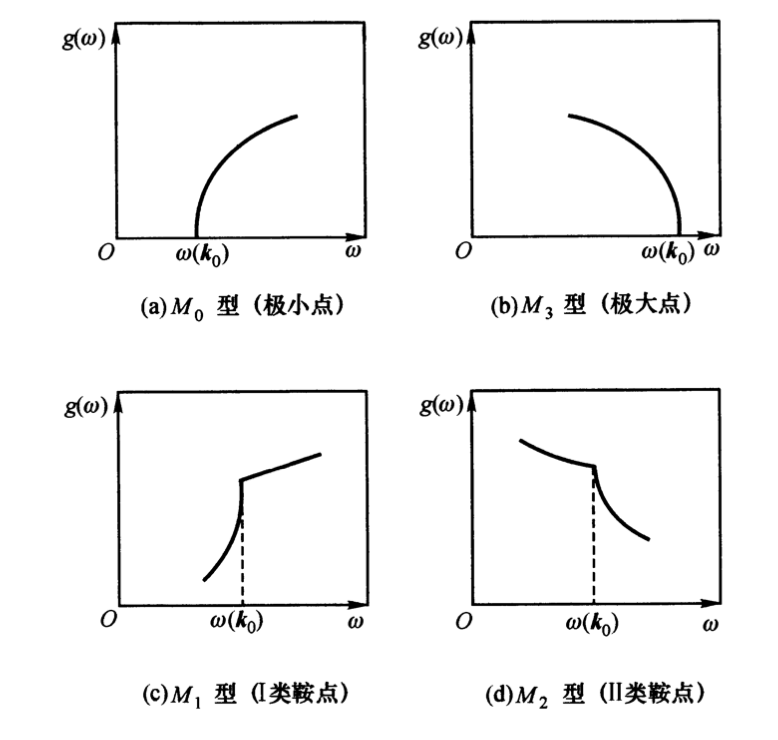
\includegraphics[height=8cm]{figures/fanhuofu.png}
\caption{四类范霍夫奇点及其相应态密度行为特点}
\label{fig:fanhuofu}
\end{center}
\end{figure}
\subsection{晶格振动的局域模}
考虑以为原子链,原子链中在原点处有一个杂质,其质量为$M'$,定义:
\[\epsilon=\frac{M-M'}{M}\]
$\epsilon$就刻画了杂质的情况,小于零时代表重杂质,大于零时代表轻杂质。这时系统的动能和势能项分别为:
\[T=\frac{1}{2}M\sum_{l}\dot{u}_l^2+\frac{1}{2}(M'-M)\dot{u}_0^2\]
\[V=\frac{1}{2}f\sum_l(u_l-u_{l+1})^2\]
利用布洛赫波函数将原子的振动位移展开:
\[u_l=\frac{1}{\sqrt{N}}\sum_k\xi_ke^{-ikla}\]
假设$\xi_k\sim e^{-i\omega t}$,那么可以得到关于震动频率的方程:
\[1=\frac{\epsilon \omega^2}{N}\sum_k\frac{1}{\omega^2-\omega_M^2}=F(\omega)\]
因此画出函数$F(\omega)$,那么便可以通过作图得到原子振动的频率,最后的结果如图\ref{fig:juyumo}所示。由图可知,重杂质情形在声频带许可的范围内,非完整晶格的震动频率向低频移动,并且与完整晶格的简正模解有一个一一对应关系。对于轻杂质情形,非完整晶格的震动频率向高频移动,非完整晶格的解比完整晶格解少一个,这个成为局域振动模式,在$\omega>\omega_M$的频带内。\par
\begin{figure}
\begin{center}
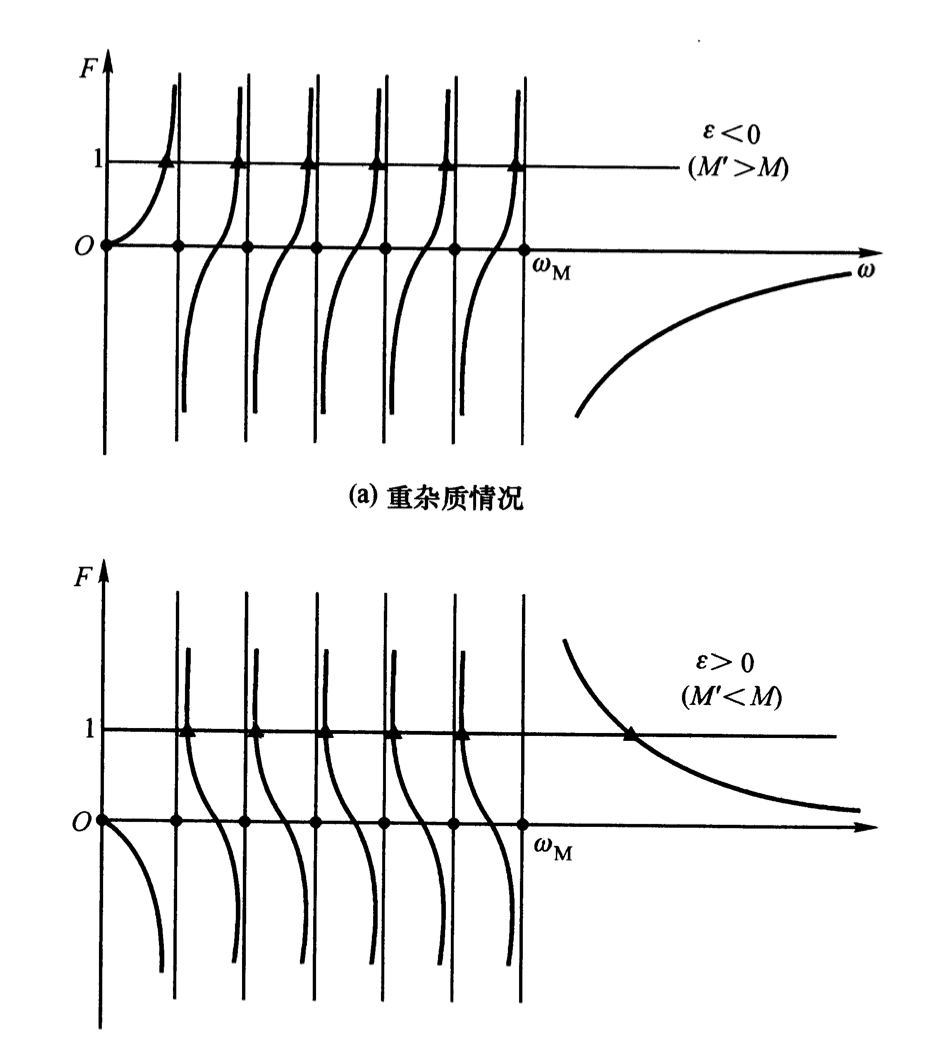
\includegraphics[height=8cm]{figures/juyumo.png}
\caption{重杂质与轻杂质情形得到的系统的振动频率与无缺陷时的比较图}
\label{fig:juyumo}
\end{center}
\end{figure}

